%%%%%%%%%%%%%%%%%%%%%%%%%%%%%%%%%%%%%%%%%%%%%%%%%%%%%%%%%%%%%%%%%%%%%%%%%%%%%%%%
% AMS Beamer series / Bologna FC / Template
% Andrea Omicini
% Alma Mater Studiorum - Università di Bologna
% mailto:andrea.omicini@unibo.it
%%%%%%%%%%%%%%%%%%%%%%%%%%%%%%%%%%%%%%%%%%%%%%%%%%%%%%%%%%%%%%%%%%%%%%%%%%%%%%%%
%\documentclass[handout]{beamer}\mode<handout>{\usetheme{default}}
%
\documentclass[presentation, 8pt]{beamer}\mode<presentation>{\usetheme{AMSBolognaFC}}
%\documentclass[handout]{beamer}\mode<handout>{\usetheme{AMSBolognaFC}}
%%%%%%%%%%%%%%%%%%%%%%%%%%%%%%%%%%%%%%%%%%%%%%%%%%%%%%%%%%%%%%%%%%%%%%%%%%%%%%%%
\usepackage[T1]{fontenc}
\usepackage{wasysym}
\usepackage{amsmath,blkarray}
\usepackage{centernot}
\usepackage{fontawesome}
\usepackage{fancyvrb}
\usepackage{tasks}
\usepackage{minted}
\usepackage{listings}
\usepackage[ddmmyyyy]{datetime}
\renewcommand{\dateseparator}{}
\usemintedstyle{tango}
\setminted{frame=lines}
%\renewcommand{\thefootnote}{\fnsymbol{footnote}}
\newcommand{\version}{1}
\usepackage{xcolor}

\definecolor{dkgreen}{rgb}{0,0.6,0}
\definecolor{gray}{rgb}{0.5,0.5,0.5}
\definecolor{mauve}{rgb}{0.58,0,0.82}
\usepackage[
	backend=biber,
	citestyle=authoryear-icomp,
	maxcitenames=1,
	bibstyle=alphabetic]{biblatex}
\lstdefinestyle{scala}{
	language=scala,
	aboveskip=3mm,
	belowskip=3mm,
	showstringspaces=false,
	columns=flexible,
	basicstyle={\ttfamily},
	numbers=none,
	numberstyle=\tiny\color{gray},
	keywordstyle=\color{blue},
	commentstyle=\color{dkgreen},
	stringstyle=\color{mauve},
	breaklines=true,
	breakatwhitespace=true,
	tabsize=2,
}

\makeatletter
\addbibresource{biblio.bib}
%%%%%%%%%%%%%%%%%%%%%%%%%%%%%%%%%%%%%%%%%%%%%%%%%%%%%%%%%%%%%%%%%%%%%%%%%%%%%%%%
\title[Multi-Agent Reinforcement Learning]
{Multi-Agent Reinforcement Learning}
%
\subtitle[]{Unleashing Collective Intelligence}
%
\author[\sspeaker{Aguzzi}]
{\speaker{Gianluca Aguzzi} \href{mailto:gianluca.aguzzi@unibo.it}{gianluca.aguzzi@unibo.it}}
%
\institute[DISI, Univ.\ Bologna]
{Dipartimento di Informatica -- Scienza e Ingegneria (DISI)\\\textsc{Alma Mater Studiorum} -- Universit{\`a} di Bologna}
%
\renewcommand{\dateseparator}{/}
\date[\today]{\today}

%
\AtBeginSection[]
{
  \begin{frame}
  \frametitle{Contents}
  \tableofcontents[currentsubsection, 
	sectionstyle=show/shaded, 
	subsectionstyle=show/shaded]
  \end{frame}
}
\AtBeginSubsection[]
{
  \begin{frame}
  \frametitle{Contents}
  \tableofcontents[currentsubsection, 
	sectionstyle=show/shaded, 
	subsectionstyle=show/shaded]
  \end{frame}
}
%
%%%%%%%%%%%%%%%%%%%%%%%%%%%%%%%%%%%%%%%%%%%%%%%%%%%%%%%%%%%%%%%%%%%%%%%%%%%%%%%%
\begin{document}
%%%%%%%%%%%%%%%%%%%%%%%%%%%%%%%%%%%%%%%%%%%%%%%%%%%%%%%%%%%%%%%%%%%%%%%%%%%%%%%%

%/////////
\frame{\titlepage}
%/////////

%%===============================================================================
\section*{Outline}
%%===============================================================================

%/////////
\begin{frame}[c]{Multi-Agent Reinforcement Learning (MARL)}
%/////////

\begin{exampleblock}{Definition}
	\emph{Multiple} agents \textbf{learn} to take the \emph{right} actions (\textbf{policy}) to maximise a \emph{reward} signal.
\end{exampleblock}

\begin{alertblock}{Applications}
	\begin{tasks}(2)
		\task Videogames
		\task Trafic Control
		\task Robotics (\emph{Swarm robotics})
		\task Trading
		\task Energy Management
		\task Environmental Monitoring
	\end{tasks}
\end{alertblock}
\begin{exampleblock}{Today Outline}
	\begin{itemize}
		\item MARL differences with respect to Single Agent RL
		\item MARL classification
		\begin{itemize}
			\item[\faArrowRight] Cooperative vs. Competitive agents
			\item[\faArrowRight] Centralised vs Decentralised learning and acting
			\item[\faArrowRight] Homogeneous vs Heterogeneous agents
		\end{itemize}
		\item Reference to MARL algorithms
		\item Scale to \textbf{infinity}: MARL large scale applications
		%\item Repositories: 
		%	\href{https://github.com/cric96/pc-multi-agent-modelling}{\faLink}
		%	\href{https://github.com/cric96/swarm-rl-alchemist}{\faLink}

	\end{itemize}
\end{exampleblock}
\end{frame}
\begin{frame}{Motivating Examples}
\centering
\begin{exampleblock}{OpenAI Hide And Seek: \url{https://openai.com/blog/emergent-tool-use/}}
	\begin{figure}
		\href{https://www.youtube.com/watch?v=kopoLzvh5jY}{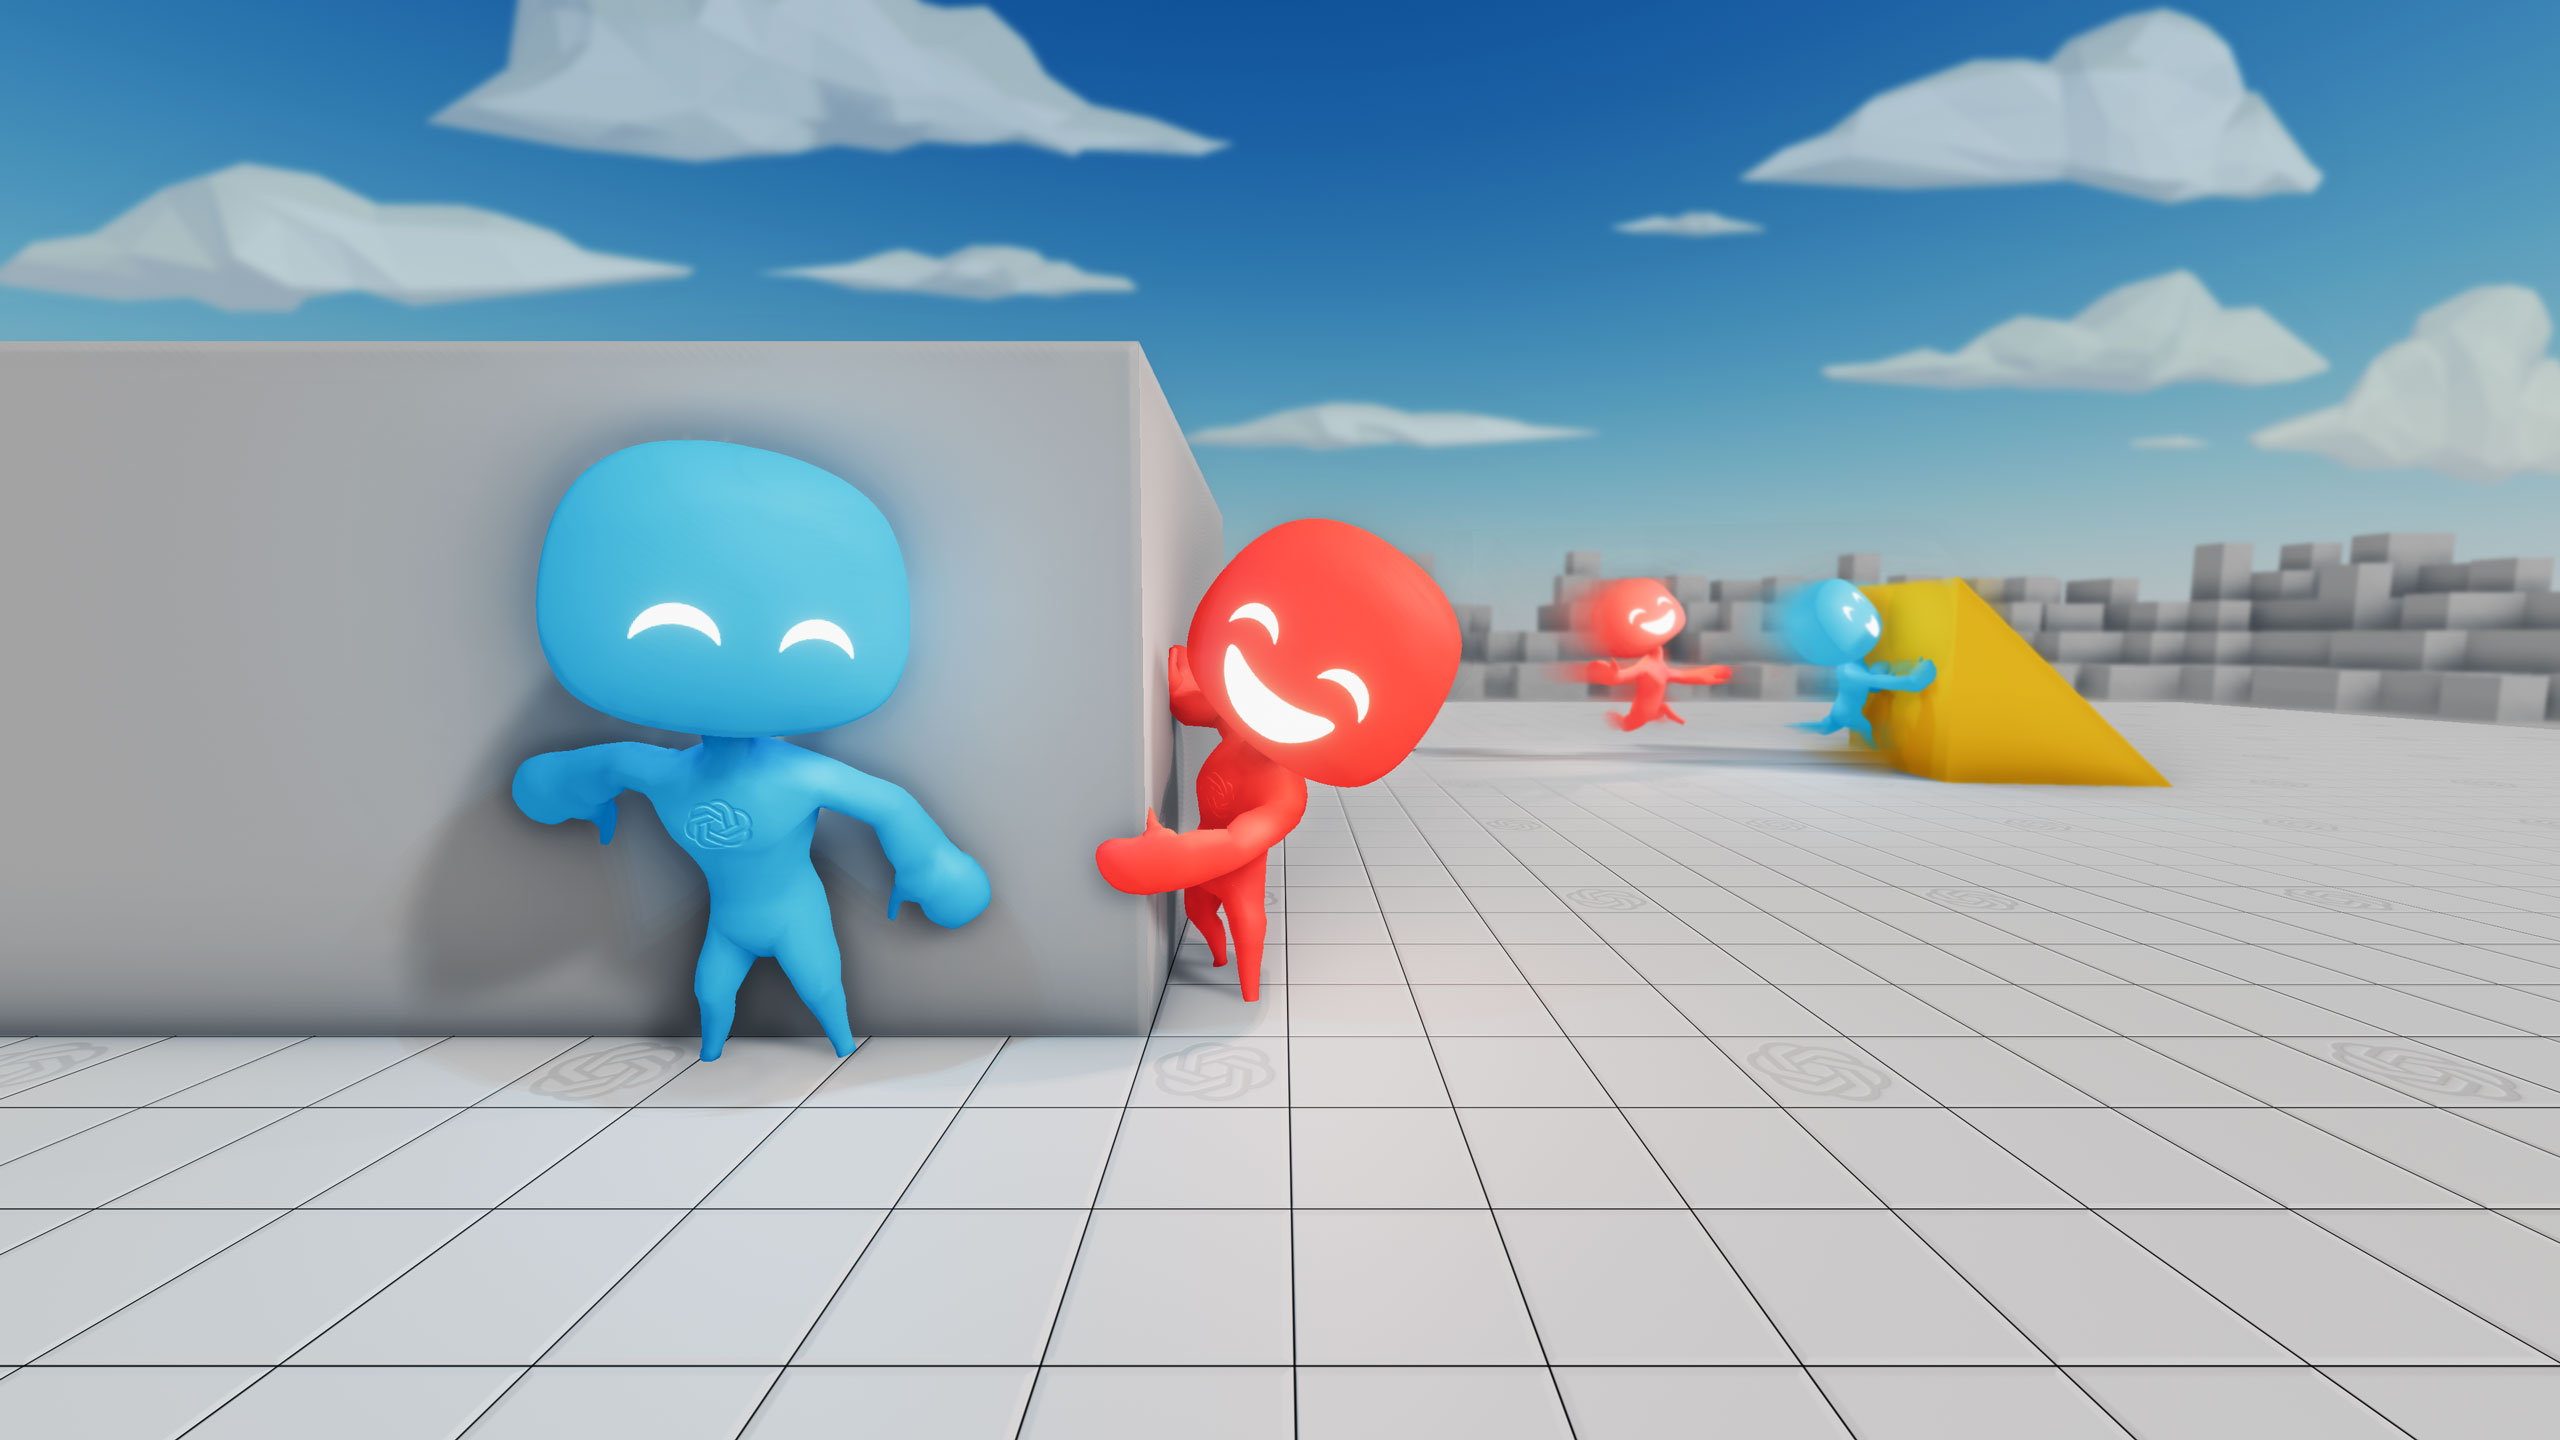
\includegraphics[width=\textwidth]{img/open-ai.jpg}}
	\end{figure}
\end{exampleblock}
\end{frame}
\begin{frame}{Motivating Examples}
\begin{exampleblock}{Capture The Flag: \url{https://deepmind.com/blog/article/capture-the-flag-science}}
	\begin{figure}
		\centering
		\href{https://www.youtube.com/watch?v=dltN4MxV1RI}{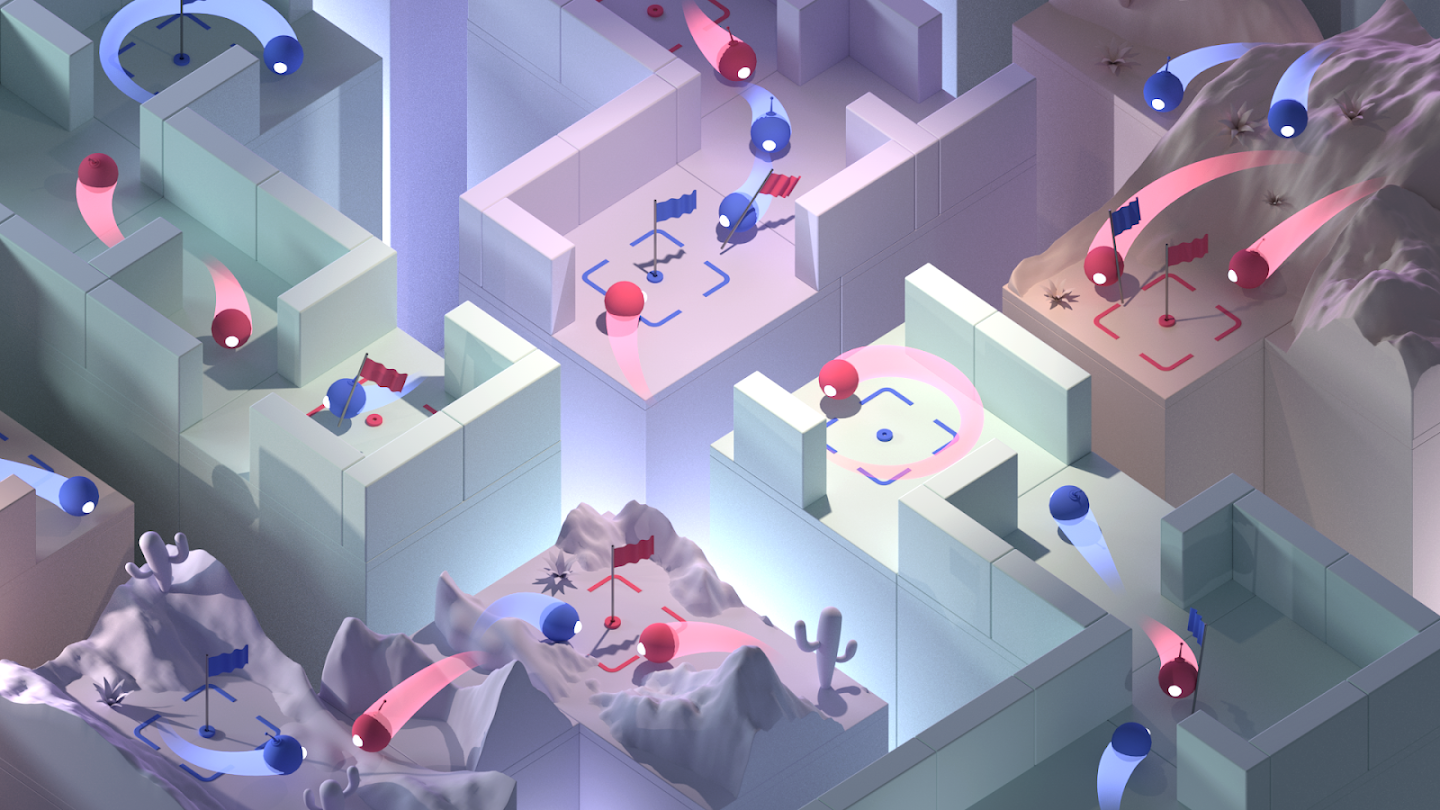
\includegraphics[width=0.85\textwidth]{img/capture-the-flag.png}}
	\end{figure}	
\end{exampleblock}
\end{frame}
\begin{frame}{Motivating Examples}
	\begin{exampleblock}{Robot Collision Avoidance}
		\centering
		\begin{figure}
			\href{https://www.youtube.com/watch?v=Uj1yAmlL5lk}{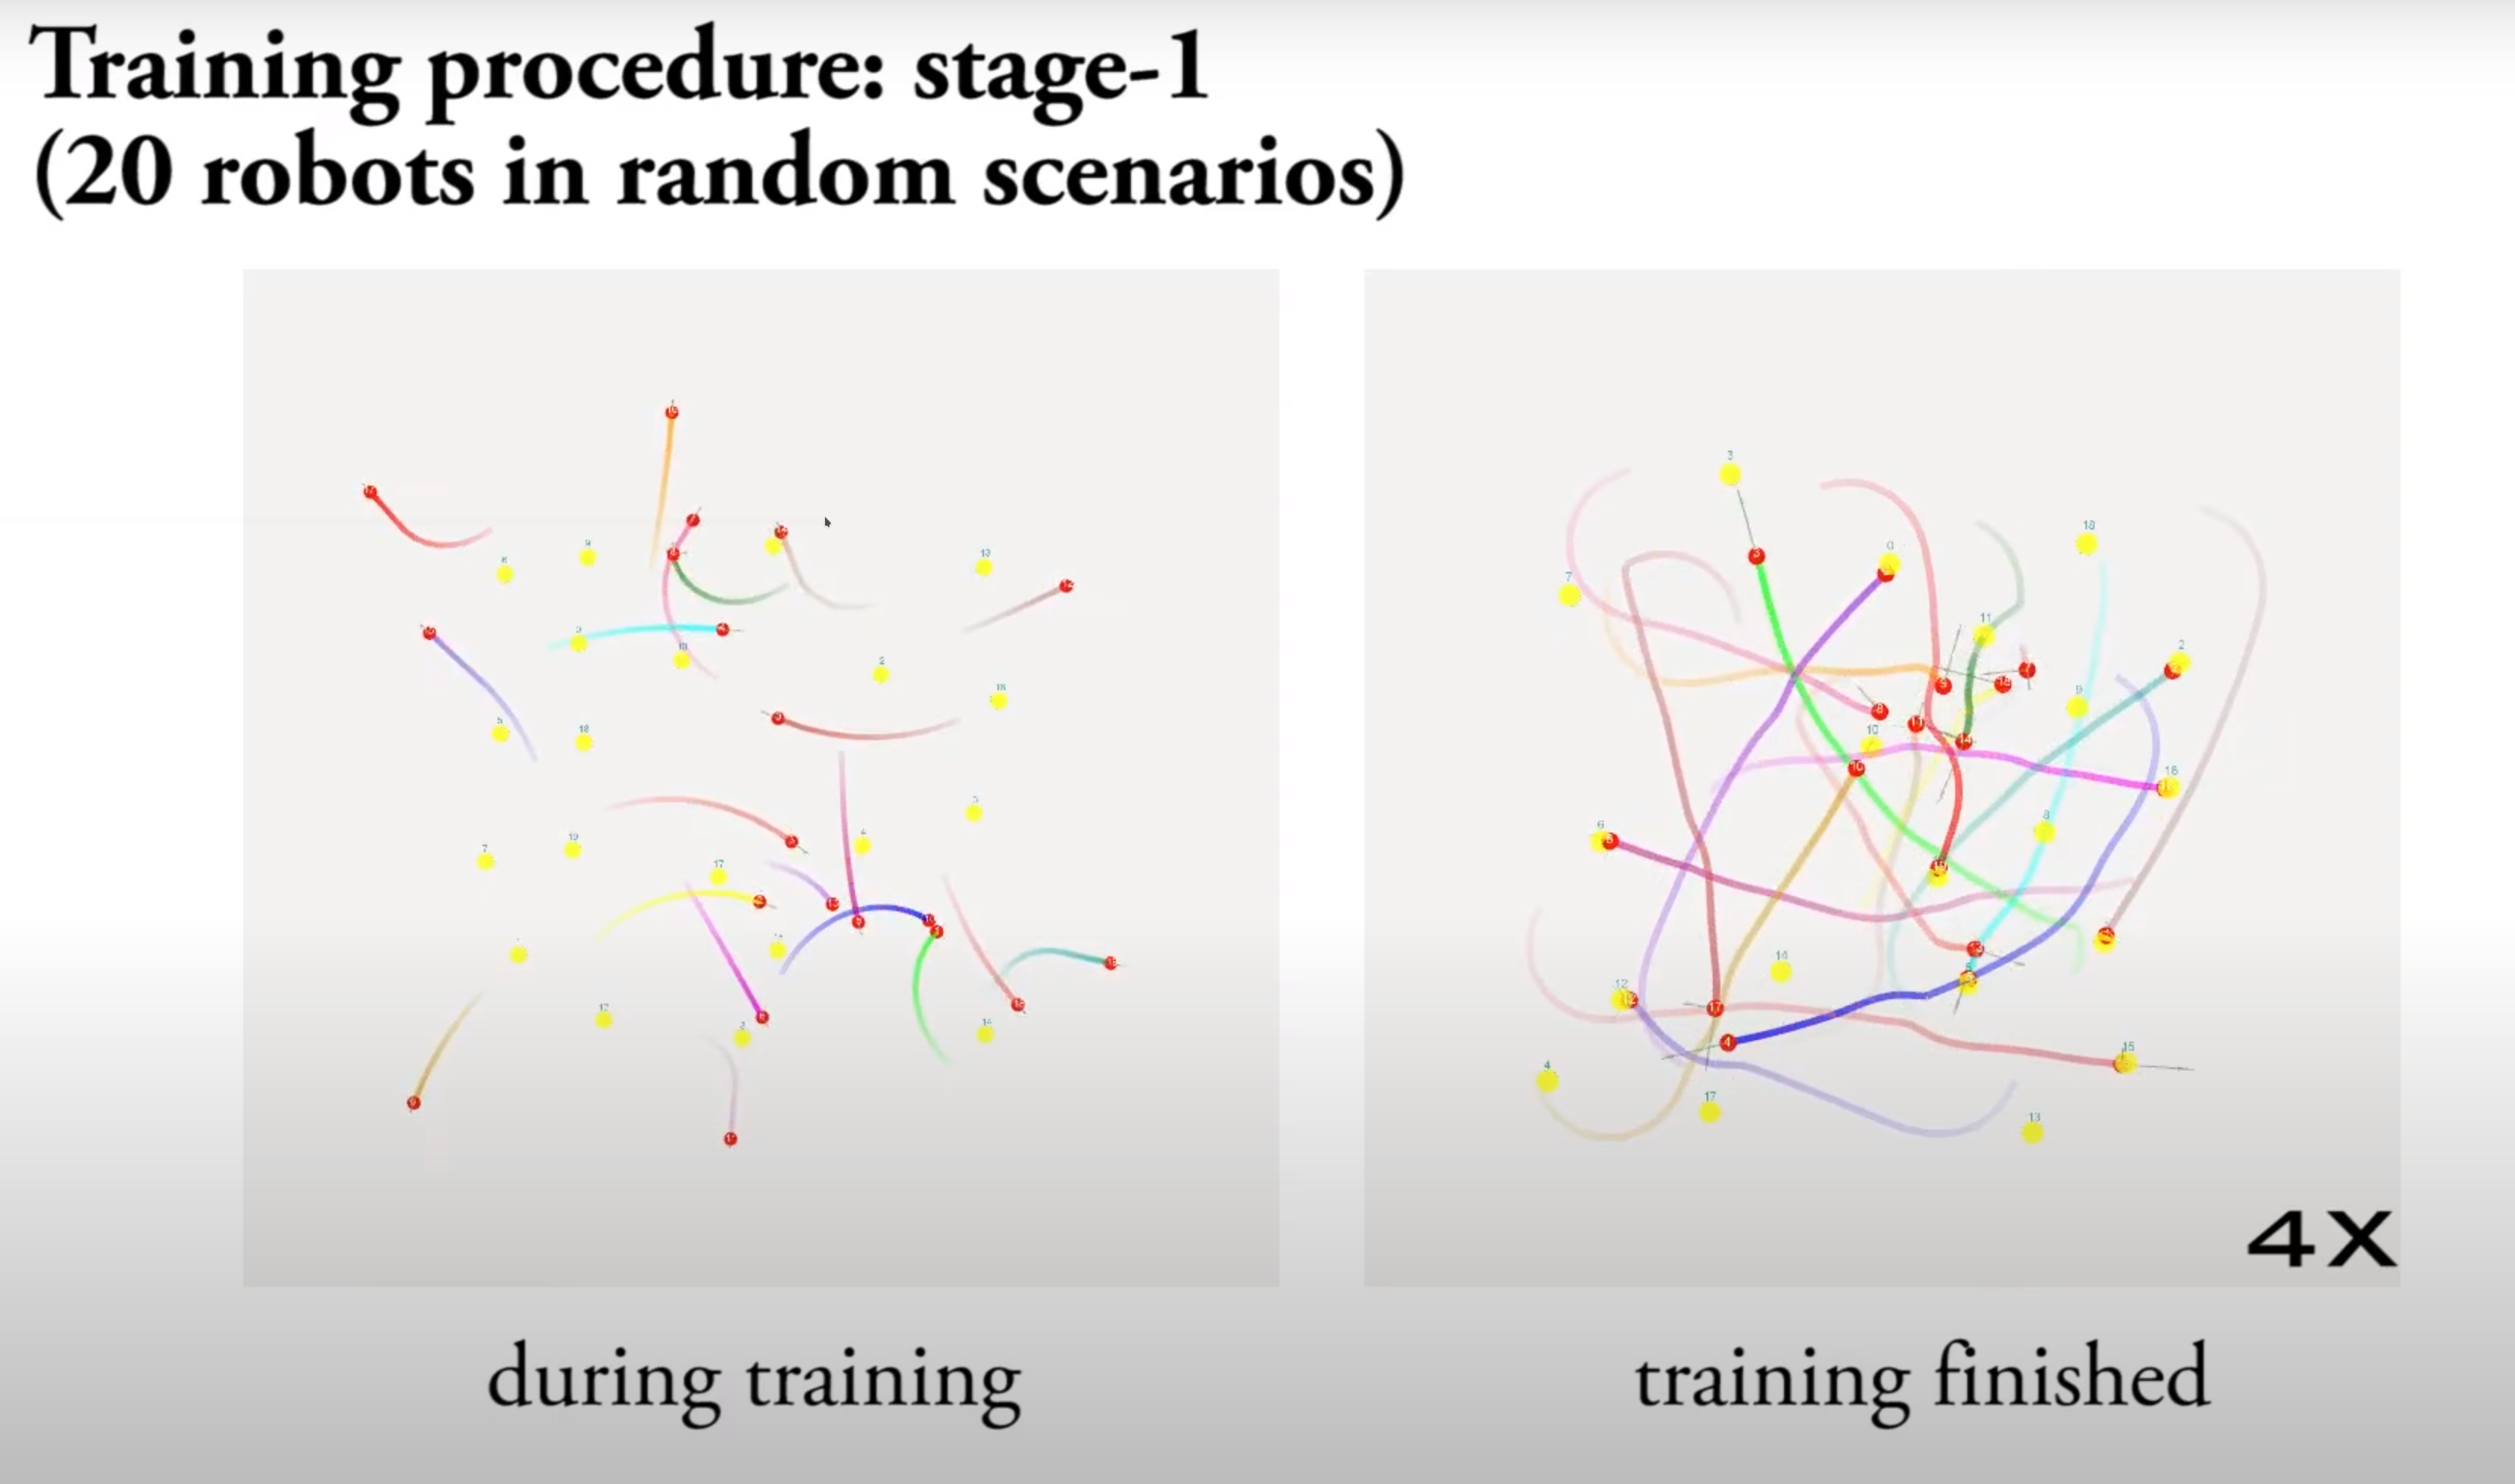
\includegraphics[width=0.7\textwidth]{img/collective-learning.png}}
		\end{figure}
	\end{exampleblock}
\end{frame}
\begin{frame}{Motivating Examples}
	\begin{exampleblock}{MAgent}
		\begin{figure}
			\href{https://www.youtube.com/watch?v=HCSm0kVolqI}{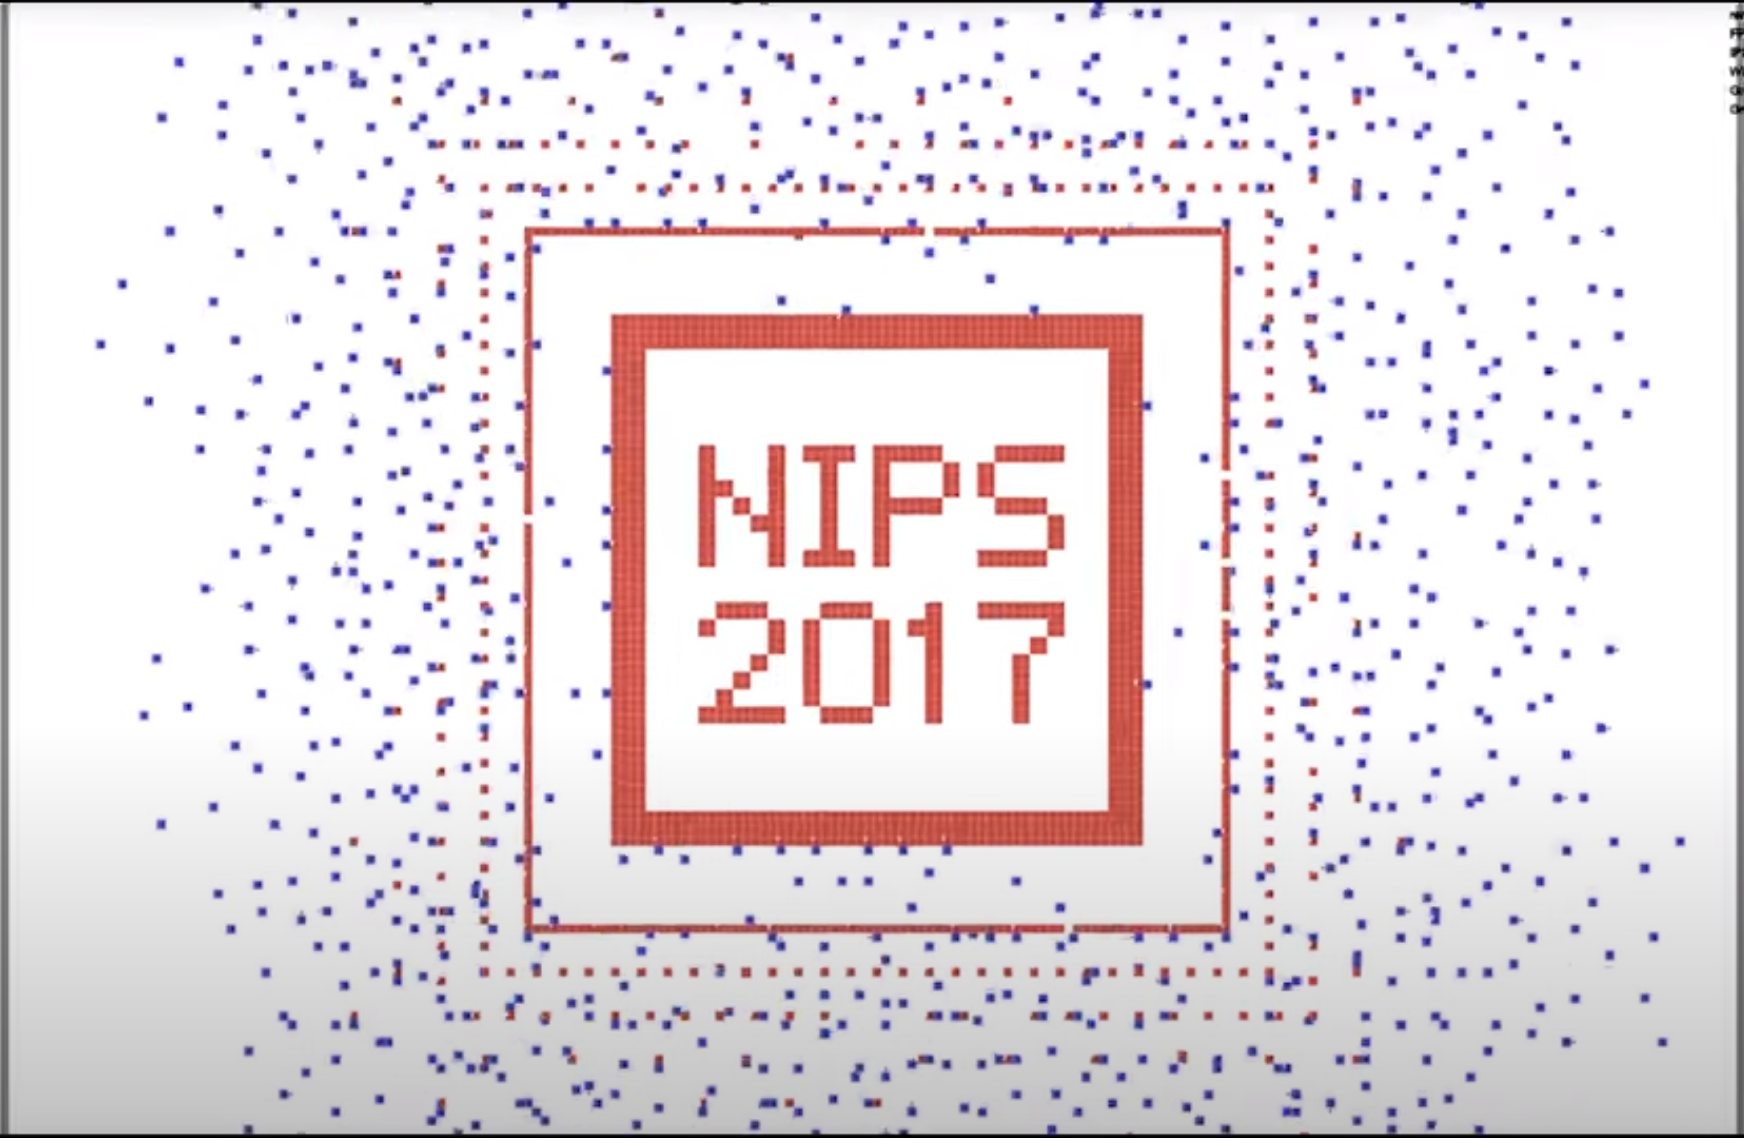
\includegraphics[width=0.7\textwidth]{img/magent.png}}
		\end{figure}
	\end{exampleblock}
\end{frame}
\begin{frame}[allowframebreaks]{Real-case applications}

\begin{exampleblock}{Trafic control reduction}
	\begin{itemize}
		\item Trafic control is an important issue in modern cities (long waiting times, accidents)
		\item Coordinating the actions of multiple agents (cars) can lead to a better overall performance
	\end{itemize}
	\centering
	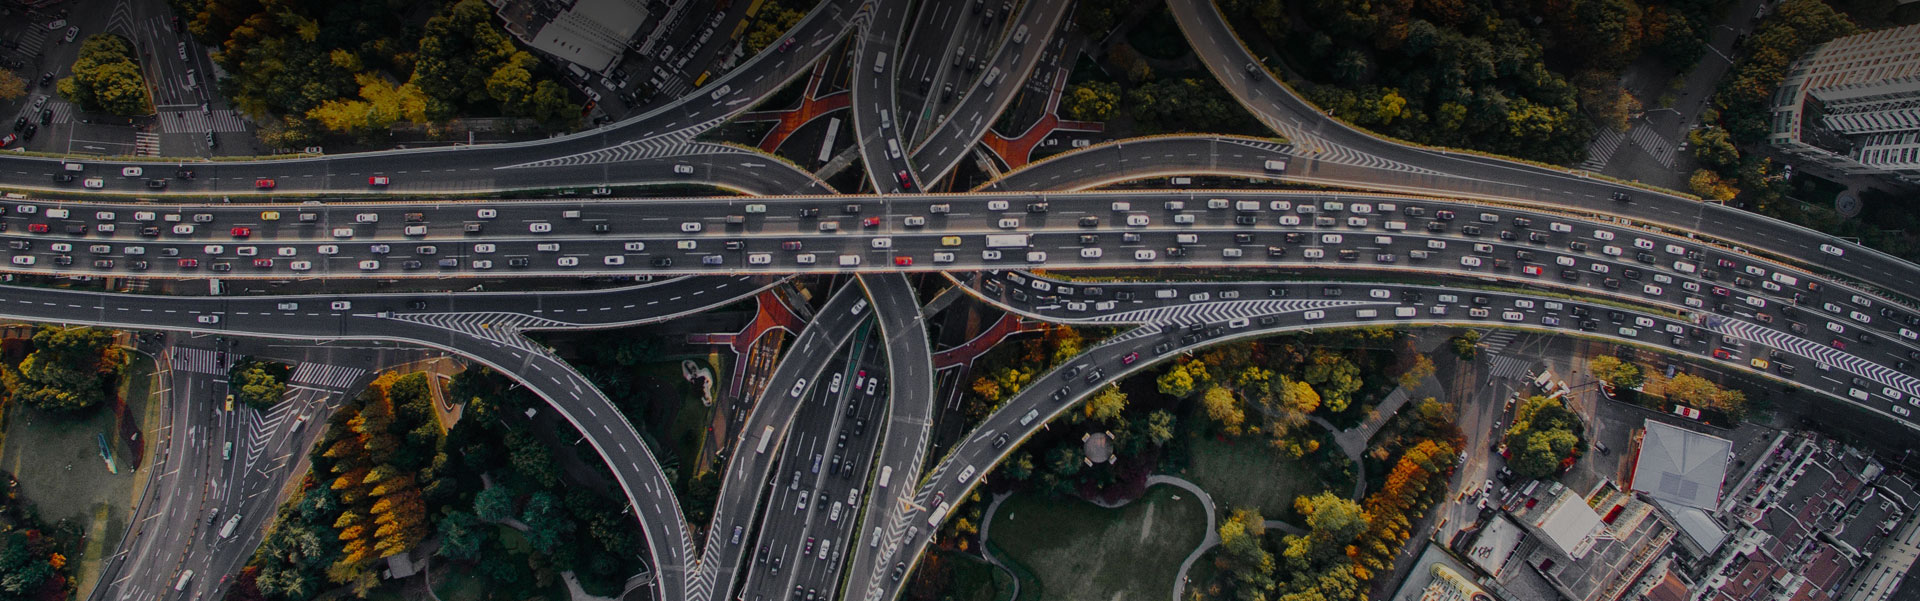
\includegraphics[width=0.38\textwidth]{img/traffic.jpg}
\end{exampleblock}
\begin{exampleblock}{Antenna tilt control}
	\begin{itemize}
		\item The joint configuration base stations can be optimized according to the distribution
	\end{itemize}
	\centering
	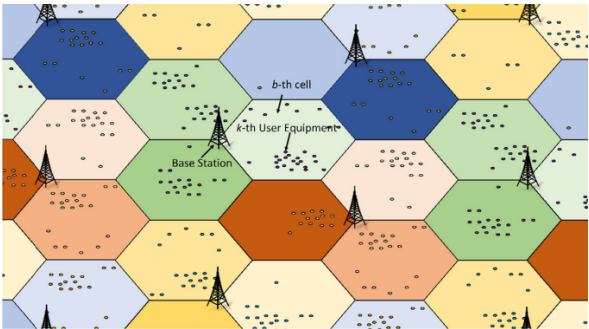
\includegraphics[width=0.4\textwidth]{img/antenna.png}
\end{exampleblock}
\end{frame}
\begin{frame}{Benefits of Multi-Agent Learning}
	\begin{itemize}
		\item \textbf{Sharing experience}
		\begin{itemize}
			\item via communication, teaching, imitation
		\end{itemize}
		\item \textbf{Parallel computation}
		\begin{itemize}
			\item due to decentralized task structure
		\end{itemize}
		\item \textbf{Robustness}
		\begin{itemize}
			\item redundancy, having multiple agents to accomplish a task
		\end{itemize}
	\end{itemize}
\end{frame}
\begin{frame}{Single Agent Reinforcement Learning}
	\begin{exampleblock}{What have you seen so far \dots}
		\begin{itemize}
			\item We have seen how to model the agent-environment interactions
			\item Find a learning process that eventually leads to an \emph{optimal} policy $\pi^*$
			\item Q-Learning (in general \emph{value-based approaches}) as a prominent algorithm to reach converge
		\end{itemize}
	\end{exampleblock}
	\begin{alertblock}{\dots But plain RL works only under some conditions}
		\begin{itemize}
			\item Full environment observability and Markovian property
			\item Stationary environment
			\item State/action space should be small enough to be stored in memory (otherwise, we should leverage function approximators)
		\end{itemize}	
	\end{alertblock}
\end{frame}

\begin{frame}{Partial Observable environments}
%/////////
	\begin{alertblock}{Definition}
		An agent does not have a \emph{perfect} and \emph{complete} knowledge of the state of the environment
	\end{alertblock}

	\begin{figure}
		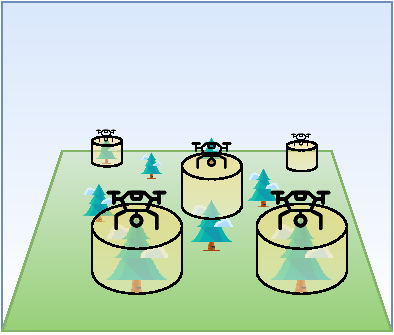
\includegraphics[height=5cm]{img/challenge-partial-observable.pdf}
	\end{figure}
\end{frame}
\begin{frame}[c]{Non-stationary environments}
	%/////////
	\begin{alertblock}{Definition}
		The environment model (e.g. the random variable associated with it) changes
		over time.
	\end{alertblock}
	\begin{exampleblock}{}
		\begin{itemize}
			\item Real-case environment dynamics could change over time (e.g. markets, city traffic, routing networks)
			\item Practically, it seems that RL (in particular Temporal Difference (TD) methods) works well even in this case
			\item \emph{But, we lose convergence guarantees.}
		\end{itemize}
	\end{exampleblock}
%
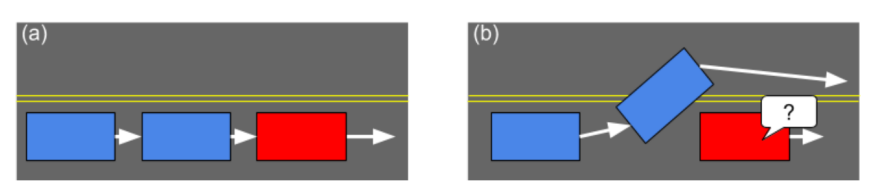
\includegraphics[width=\textwidth]{img/non-stationary.png}
\end{frame}

\begin{frame}{Agents-environment interaction}
\begin{itemize}
	\item Simple modelation:
	\begin{itemize}
		\item At each time step $t$
		\begin{itemize}
			\item Each agent $i$ observes the environment state $s_t$ (or a part of it, $o_t^i$)
			\item Each agent $i$ selects an action $a_t^i$ (possibly different from the others)
			\item The collective action is $a_t = (a_t^1, \dots, a_t^N)$ is applied to the environment
			\item The environment evolves to a new state $s_{t+1}$ and provides a reward $r_{t+1}$ to each agent
		\end{itemize}
	\end{itemize}
\end{itemize}
\centering
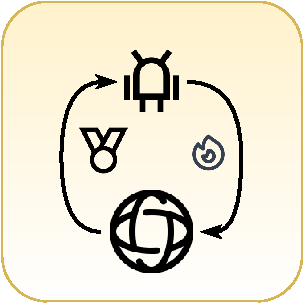
\includegraphics[width=0.4\textwidth]{img/single-agent-multi-agent-1.pdf}
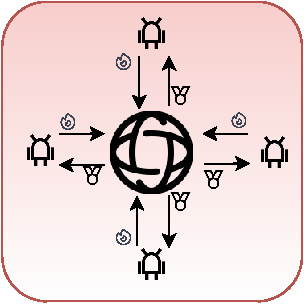
\includegraphics[width=0.4\textwidth]{img/single-agent-multi-agent-2.pdf}
\end{frame}

\begin{frame}{Multi but how many?}
	\begin{itemize}
		\item Well-studied applications \faArrowRight \, 2 agents
		\begin{itemize}
			\item mainly board games
		\end{itemize}
		\item Finite number of agents \faArrowRight \, $N$ agents
		\begin{itemize}
			\item e.g. traffic control, antenna tilt control
			\item Two-agents approaches can be extended to $N$ agents
			\item Finite but small
		\end{itemize}
		\item ``Infinite''
		\begin{itemize}
			\item Very large-scale systems
			\item We cannot know the number of agents in advance
			\item Typically referred as \emph{many} agent systems
		\end{itemize}
	\end{itemize}
\end{frame}

\begin{frame}{MARL Systems: Task type}
	%/////////
		\begin{alertblock}{Cooperative}
			\begin{itemize}
				\item Agents share the same reward function ($R^1 = \dots = R^N$) in order to accomplish a collective goal
			\end{itemize}
		\end{alertblock}
		\centering
		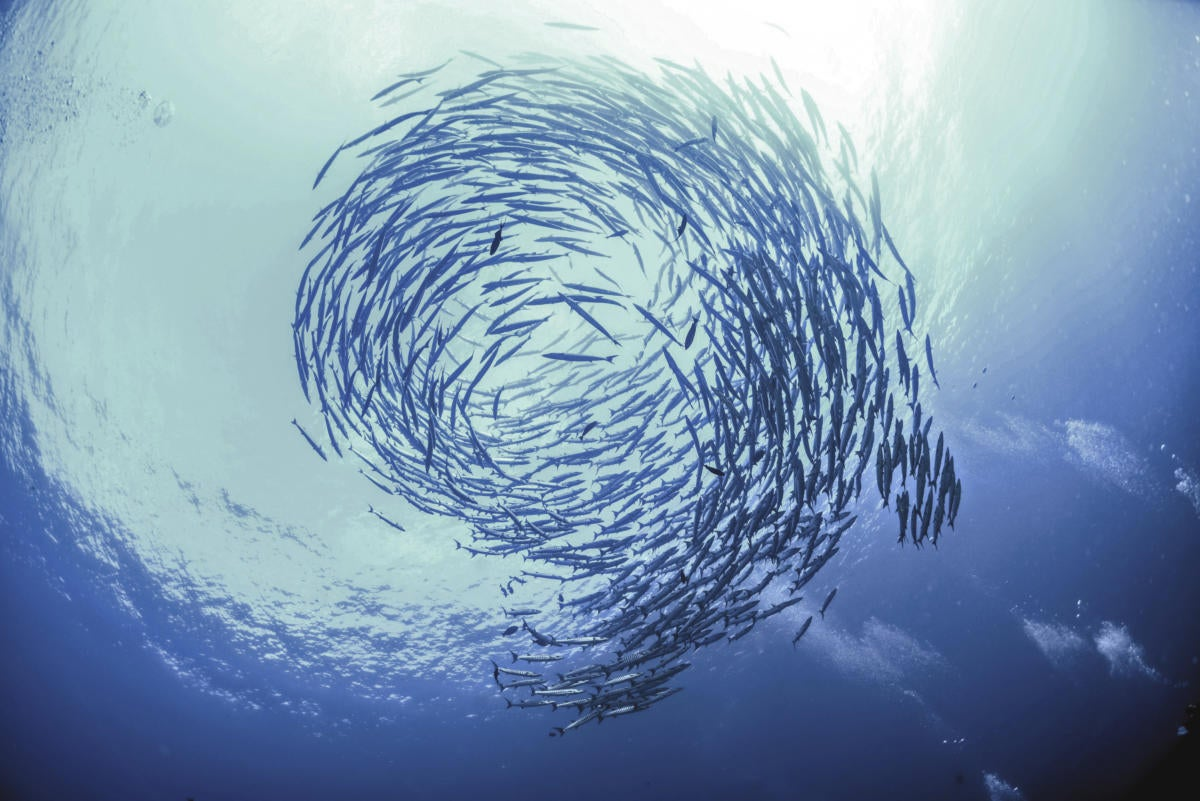
\includegraphics[height=3.5cm]{img/cooperative.jpg}
		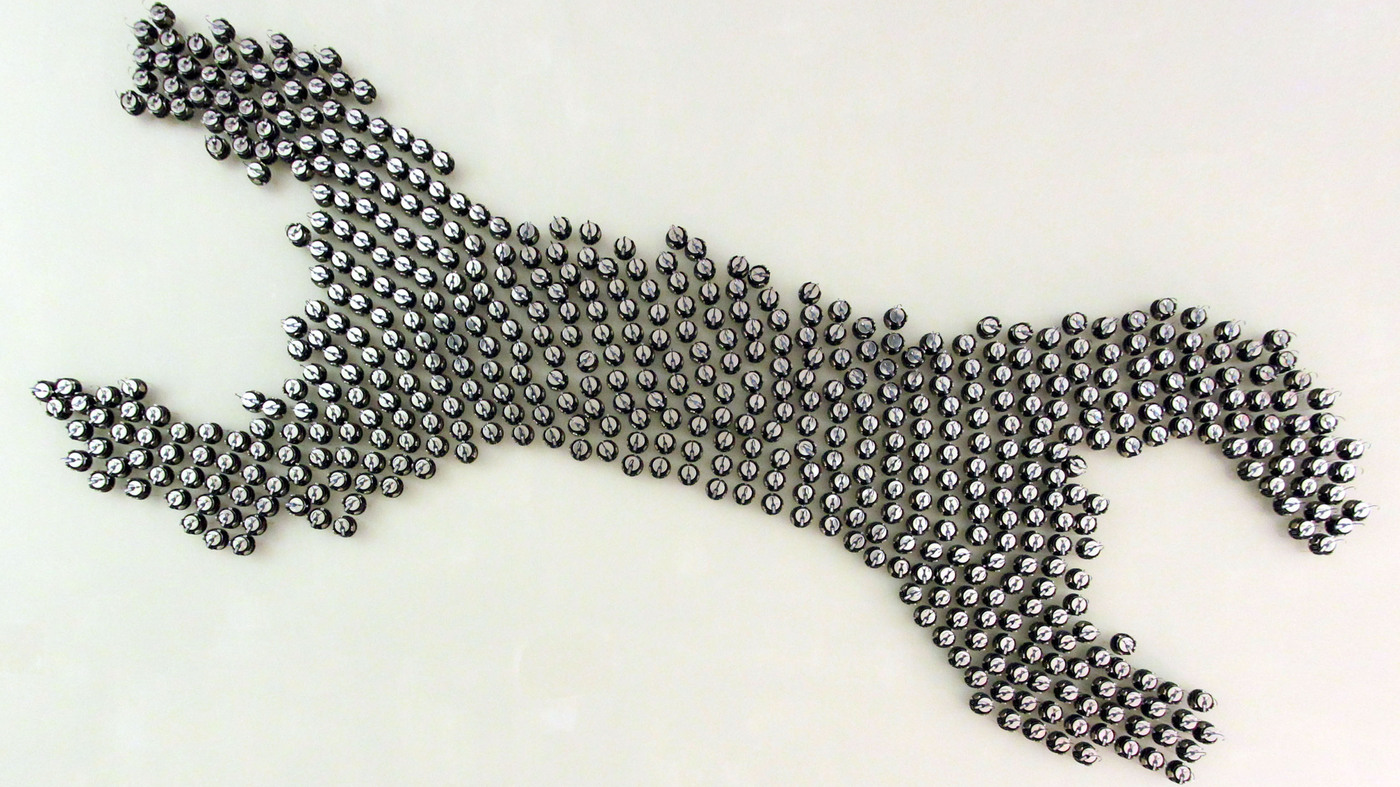
\includegraphics[height=3.5cm]{img/cas-1.jpg}
		
	\end{frame}
	
	\begin{frame}{MARL Systems: Task type}
		\begin{exampleblock}{Competitive}
			\begin{itemize}
				\item Agents compete with each other to maximise a long term return
				\item Board Games, Video games, \dots
			\end{itemize}
		\end{exampleblock}
	
		\centering
		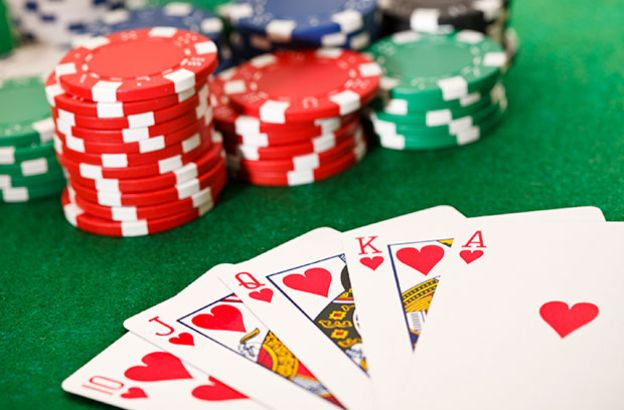
\includegraphics[height=3.5cm]{img/competitive.jpg}
		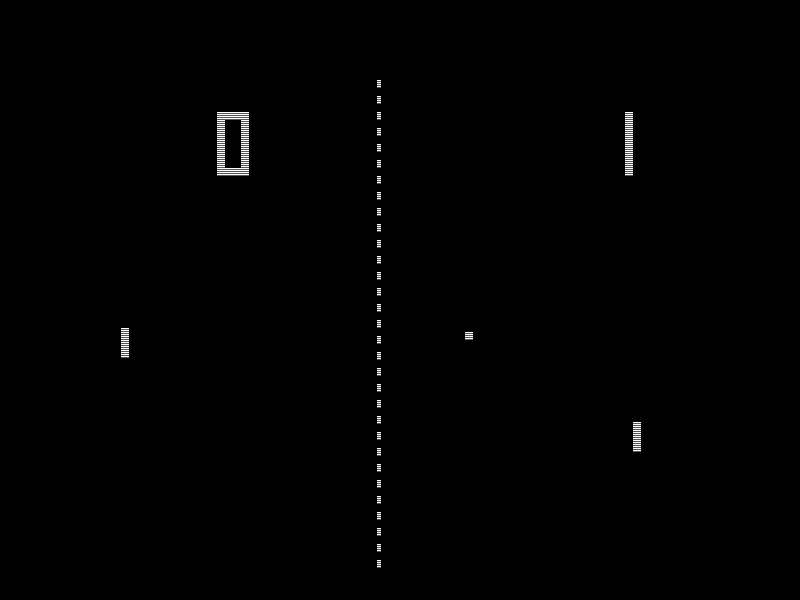
\includegraphics[height=3.5cm]{img/ping.png}
		
	\end{frame}
	
	\begin{frame}{MARL Systems: Task type}
		\begin{exampleblock}{Mixed}
			\begin{itemize}
				\item Agents can both compete and cooperate in order to maximise a global reward function
				\item Also called \textit{General Sum games}
			\end{itemize}
		\end{exampleblock}
	
		\begin{figure}
			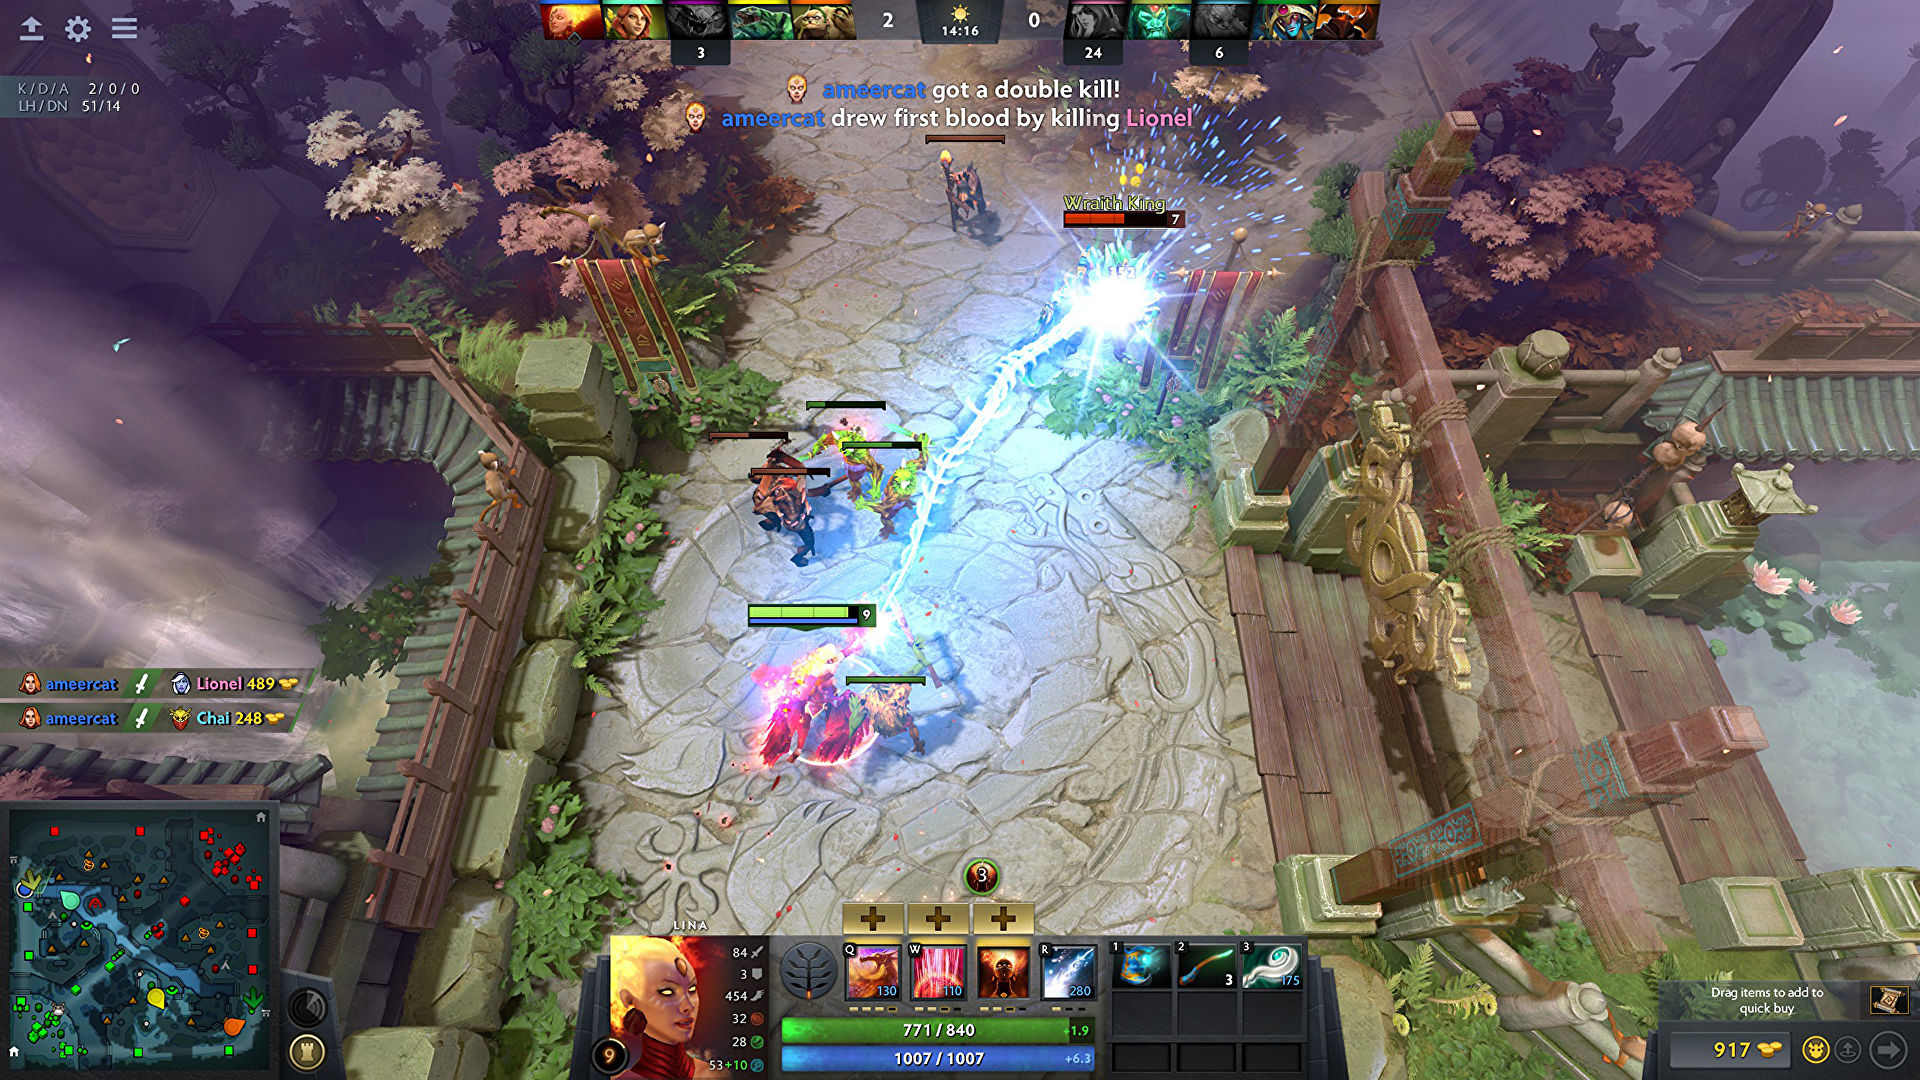
\includegraphics[height=5cm]{img/mixed}
		\end{figure}
	\end{frame}
	
	\begin{frame}{On Cooperative Task}
		\begin{exampleblock}{Homogeneous}
			\begin{itemize}
				\item Each agent has same capabilities ($A^1 = \dots = A^N$)
				\item The overall goal is to find the best policy that is the same for each agent ($\pi^* = {\pi^{*}}_1 = \pi^{*}_2 = \dots = {\pi^{*}}_N$)
			\end{itemize}
		\end{exampleblock}
		\begin{exampleblock}{Heterogeneous}
			\begin{itemize}
				\item Each agent could have different capabilities (in the worst case, $A^1 \neq \dots \neq A^N$)
				\item Each agent has its local policy that should be maximised following the global collective goal
			\end{itemize}
		\end{exampleblock}
	\end{frame}
	
	%/////////
	\begin{frame}{MARL Systems: Learning Scheme}
		\begin{exampleblock}{Centralised Training and Centralised Execution (CTCE)}
			\begin{itemize}
				\item \emph{One} agent with a global view of the system (in the cloud? or in a server?)
				\item Nodes send their perception to that central agent
				\item With these perceptions, the central node creates a global state of the system
				\item With the current policy, it chooses the actions that nodes should perform (\emph{Control})
				\item In the next time step, it evaluates the reward function and updates the policy accordingly (\emph{Learn})
				\item \emph{Are the nodes agents?}
				\item Used mainly in offline (i.e. at simulation time) setting 
			\end{itemize}
		\end{exampleblock}
	
	\end{frame}
	%/////////
	
	%/////////
	\begin{frame}{MARL Systems: Learning Scheme}
		\begin{exampleblock}{Centralised Training and Centralised Execution (CTCE)}
			\begin{figure}
				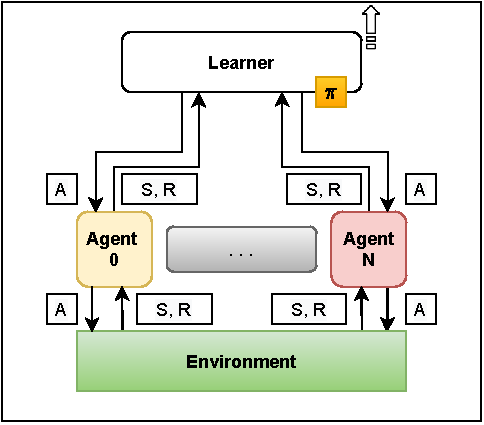
\includegraphics[height=6cm]{img/learning-scheme-clce.pdf}
			\end{figure}
		\end{exampleblock}
	\end{frame}
	%/////////
	
	%/////////
	\begin{frame}{MARL Systems: Learning Scheme}
		
		\begin{exampleblock}{Decentralised Training and Decentralised Execution (DTDE)}
			\begin{itemize}
				\item Each node has its local policy/value table
				\item They can perceive the environment state (or they can observe a part of it)
				\item With the current state, they perform an action following their local policy (\emph{Control})
				\item In the next time step, they update their policy following a local reward function (\emph{Learn})
				\item Both used in offline and online (i.e. deployment time) setting
			\end{itemize}
		\end{exampleblock}
	\end{frame}
	%/////////
	
	
	%/////////
	\begin{frame}{MARL Systems: Learning Scheme}
		\begin{exampleblock}{Decentralised Training and Decentralised Execution (DTDE)}
			\begin{figure}
				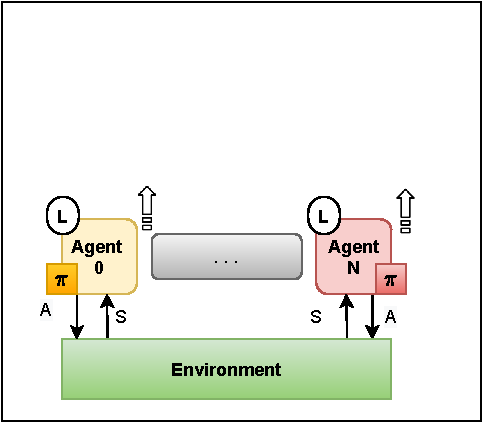
\includegraphics[height=6cm]{img/learning-scheme-dtde.pdf}
			\end{figure}
		\end{exampleblock}
	\end{frame}
	
	\begin{frame}{MARL Systems: Learning Scheme}
		
		\begin{exampleblock}{Centralised Training and Decentralised Execution (CTDE)}
			\begin{itemize}
				\item A simulation time learning online execution pattern
				\item \emph{Simulation time}
				\begin{itemize}
					\item Each node follows the typical $o_t, a_t, o_{t+1}, a_{t+1},\dots $ trajectory using a local policy
					\item After an episode, this trajectory (or something derived from it) will be sent to a central learner
					\item It, using a global view of the system, improves the policies of the agents 
					\item An then the policies will be shared with the agents
				\end{itemize} 
				\item \emph{Execution time}
					\begin{itemize}
						\item Each agent has the local policy distilled during the simulation time
						\item With it, they act in the environment
					\end{itemize}
			\end{itemize}
		\end{exampleblock}
	\end{frame}
	
	
	\begin{frame}{MARL Systems: Learning Scheme}
		\begin{exampleblock}{Decentralised Training and Decentralised Execution (DTDE)}
			\begin{figure}
				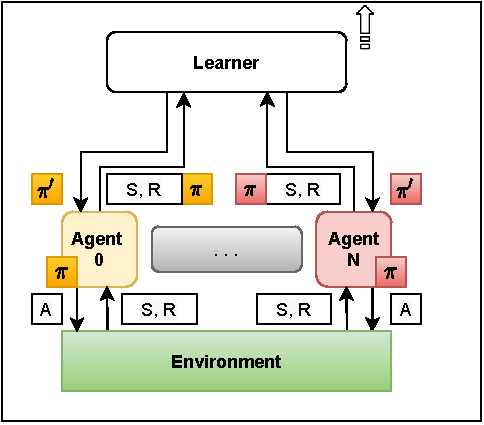
\includegraphics[height=6cm]{img/learning-scheme-ctde.pdf}
			\end{figure}
		\end{exampleblock}
	\end{frame}
\begin{frame}{Single Agent \faArrowRight \, Multi Agent}
\begin{alertblock}{Big Question: Can we use Single Agent RL in MAS?}
\begin{itemize}
	\item It depends on the \emph{task type}, \emph{policy type}, \emph{communication} constraints, \emph{execution} constraints, and \emph{learning} constraints
	\item Single agent RL could be easily adapted in some cases:
	\begin{itemize}
		\item Task type: cooperative
		\item Policy type: homogeneous
		\item Communication constraints: independent
		\item Execution constraints: centralised/decentralised
		\item Learning constraints: centralised/decentralised
	\end{itemize}
	\item What about the reward function?
	\begin{itemize}
		\item A reward function for each agent?
		\item A collective reward function?
		\item Combination?
	\end{itemize}
\end{itemize}
\end{alertblock}
\end{frame}
\begin{frame}{Independent Q Learning}
	\begin{alertblock}{Idea}
		\begin{itemize}
			\item Each agent has its own Q table
			\item Each agent improves its Q table independently following a local policy	
		\end{itemize}
	\end{alertblock}
	\begin{exampleblock}{Problems}
		\begin{itemize}
			\item The agents could learn a policy that is not optimal for the collective goal
			\item The agents could learn a policy that is not optimal for the other agents
			\item The agents could learn a policy that is not optimal for the environment
		\end{itemize}
	\end{exampleblock}
	\begin{columns}
		\begin{column}[b]{0.5\textwidth}
			\href{https://www.youtube.com/watch?v=nn6_GUVDnVw&list=PLfLv_F3r0TwyaZPe50OOUx8tRf0HwdR_u&index=2}{
				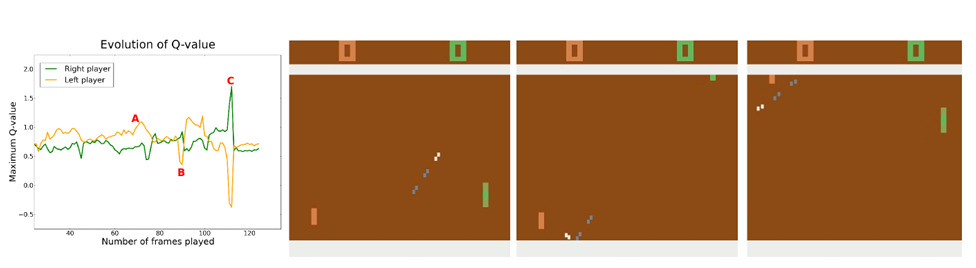
\includegraphics[width=\textwidth]{img/competitive.png}}
					
		\end{column}
		\begin{column}[b]{0.5\textwidth}
			\href{https://www.youtube.com/watch?v=Gb9DprIgdGw&list=PLfLv_F3r0TwyaZPe50OOUx8tRf0HwdR_u&index=1}{
				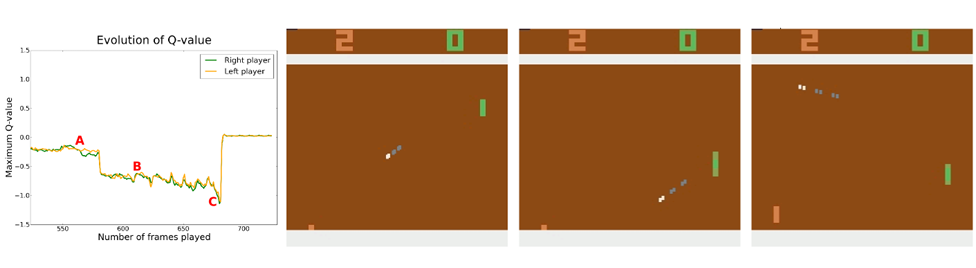
\includegraphics[width=\textwidth]{img/cooperative.png}}
					
		\end{column}
	\end{columns}
\end{frame}
\begin{frame}{COMA}
	\begin{itemize}
		\item COMA (Counterfactual Multi-Agent) is a technique that uses a \emph{centralised} training and a \emph{decentralised} execution
		\item Idea: ease the learning processes by giving a \emph{global} view of the environment 
		\item Counterfactual baseline: a baseline that is independent of the actions taken by the agent
		\begin{itemize}
			\item Used to understand the impact of the agent's actions
		\end{itemize}
	\end{itemize}
	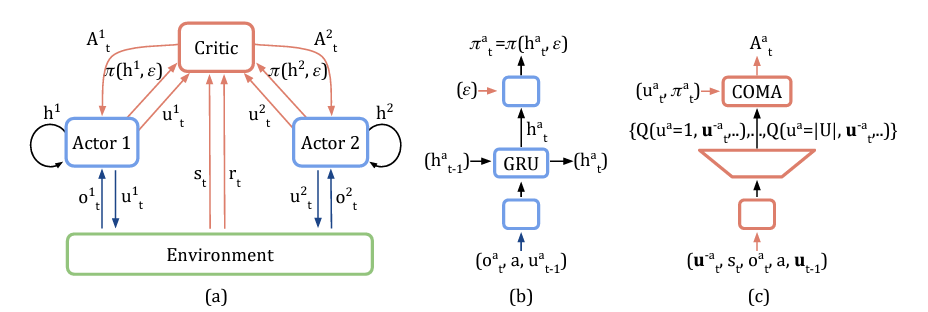
\includegraphics[width=\textwidth]{img/coma.png}
\end{frame}
\begin{frame}{Learning to Communicate}
	\begin{itemize}
		\item The agent coordination can be ruled via \emph{communication}
		\item This communication can be learned through \emph{reinforcement learning}
	\end{itemize}
	\centering
	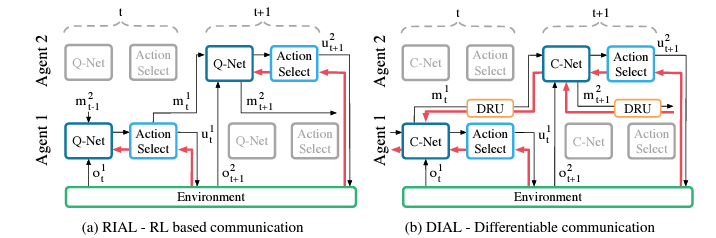
\includegraphics[width=\textwidth]{img/learning-to-communicate.png}
\end{frame}
\begin{frame}{MAPPO}
	\begin{itemize}
		\item MAPPO (Multi-Agent Proximal Policy Optimisation) is the extension of PPO to MARL
		\begin{itemize}
			\item Promising results in cooperative and competitive tasks with few agents
		\end{itemize}
	\end{itemize}
	\centering
	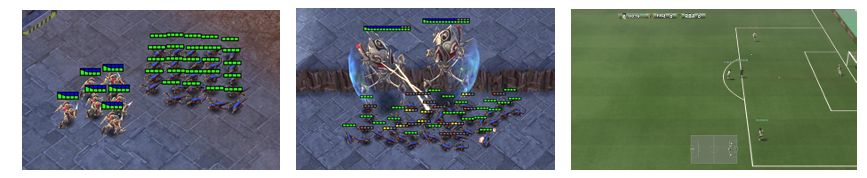
\includegraphics[width=\textwidth]{img/mappo.png}
\end{frame}
\begin{frame}{Decentralised Hysteretic Deep-Recurrent-Q Learning}
	\begin{itemize}
		\item The previous approach suppose to have a centralised controller
		\item cons:
		\begin{itemize}
			\item offline learning
			\item hard to scale (without weight sharing)
		\end{itemize}
		\item Decentralised Hysteretic Deep-Q Learning (DH-DQL) is a technique that uses a \emph{decentralised} training and a \emph{decentralised} execution
		\item The agents maximise a local reward function
		\begin{itemize}
			\item Collective goal reached by emergent behaviour
		\end{itemize}
		\item Strategies:
		\begin{itemize}
			\item \emph{Hysteretic}: heuristic that prevents the agents to change their policy too often bringing in miscoordination
			\item \emph{Recurrent Neural Network}: to manage the partial observability
		\end{itemize}
	\end{itemize}
\end{frame}

\begin{frame}{Learning in Many Agent Systems}
	\begin{alertblock}{Problems}
		\begin{itemize}
			\item Many Agent Systems are challenging environments for learning
			\begin{itemize}
				\item The agents involved could be hundreds or thousands
				\item The state space could be very large
				\item The agents only have partial information about the state
				\item No central controller (at runtime)
			\end{itemize}
		\end{itemize}
	\end{alertblock}
	\begin{alertblock}{How?}
		\begin{itemize}
			\item Constraints on policy: \emph{homogeneous}
			\begin{itemize}
				\item The \textbf{complexity} emerges through interactions
			\end{itemize}
			\item Partial observability handled through \emph{deep learning} (e.g., Deep Q-Learning)
			\item Centralised training and decentralised execution strategy
			\begin{itemize}
				\item During the simulation the agents are trained using a centralised training algorithm
				\item The Q table is local to each agent
				\item After the simulation, it will be copied into each agent
				\item No need for a central controller at runtime!
			\end{itemize}
			\item Communication handled through \emph{message passing} and encoded as a local state
			\item \emph{Dense} reward to simplify the learning process and to enable cooperation
		\end{itemize}
	\end{alertblock}
\end{frame}
\begin{frame}{Mean-field Reinforcement Learning}
	\begin{itemize}
		\item \textbf{Mean-field} Reinforcement Learning (MRL) is a technique to reduce the complexity of a multi-agent system
		\item The idea is to approximate the behaviour of the agents as a single agent (i.e., the \textbf{mean-field} agent)
	\end{itemize}
	\centering
	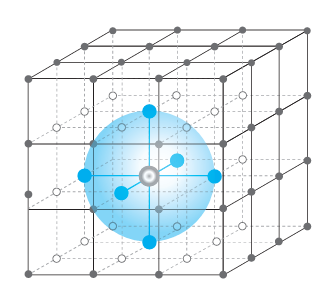
\includegraphics[width=0.45\textwidth]{img/mean-field.png}
	\centering
	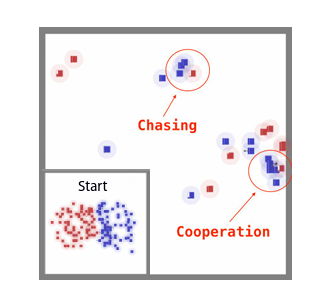
\includegraphics[width=0.45\textwidth]{img/result-mean-field.png}
\end{frame}
	\begin{frame}{Field-Informed Multi-Agent Reinforcement Learning}
		\begin{itemize}
			\item Field-Informed MARL is a technique that guides the learning process of the agents using a \emph{computational} field
			\item Idea: ease the learning process by providing a \emph{prior} knowledge about the environment
		\end{itemize}
		\centering
		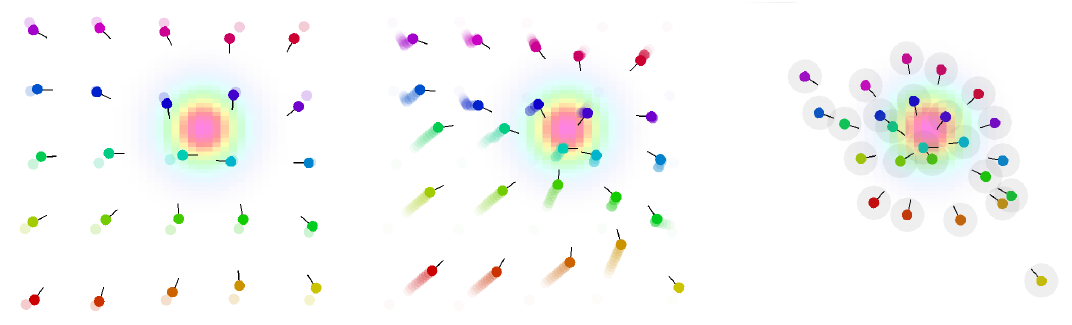
\includegraphics[width=0.8\textwidth]{img/field-informed.png}
		\centering
		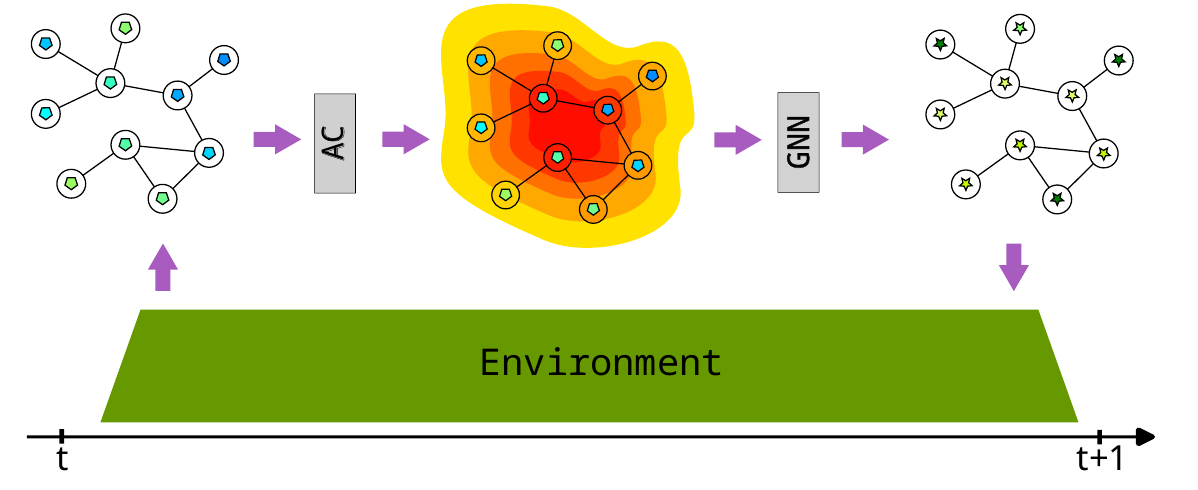
\includegraphics[width=0.8\textwidth]{img/field-informed-schema.png}
	\end{frame}

\begin{frame}{Example: Follow the leader}
\begin{exampleblock}{Scenario}
	\begin{itemize}
		\item Configuration: N agents, M neighbours, 8 directions + standstill
		\item But aggregate computing is used to share the leader towards a gradient
		\item Reward function is composed of two terms
		\begin{itemize}
			\item collision: the nearest agent distance should be as large as possible 
			\item leader: the distance to the leader should be as small as possible
		\end{itemize}
	\end{itemize}

\end{exampleblock}
\centering {
	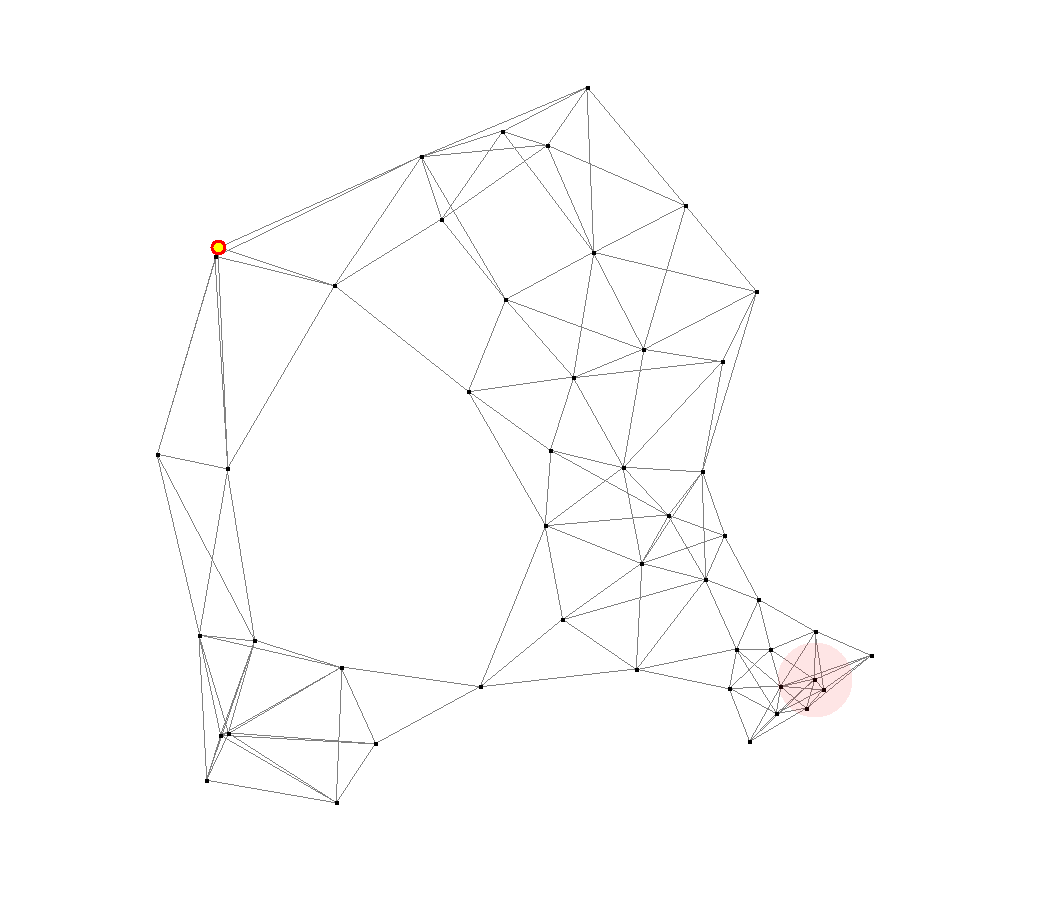
\includegraphics[width=0.3\textwidth]{img/moment-a.png}
	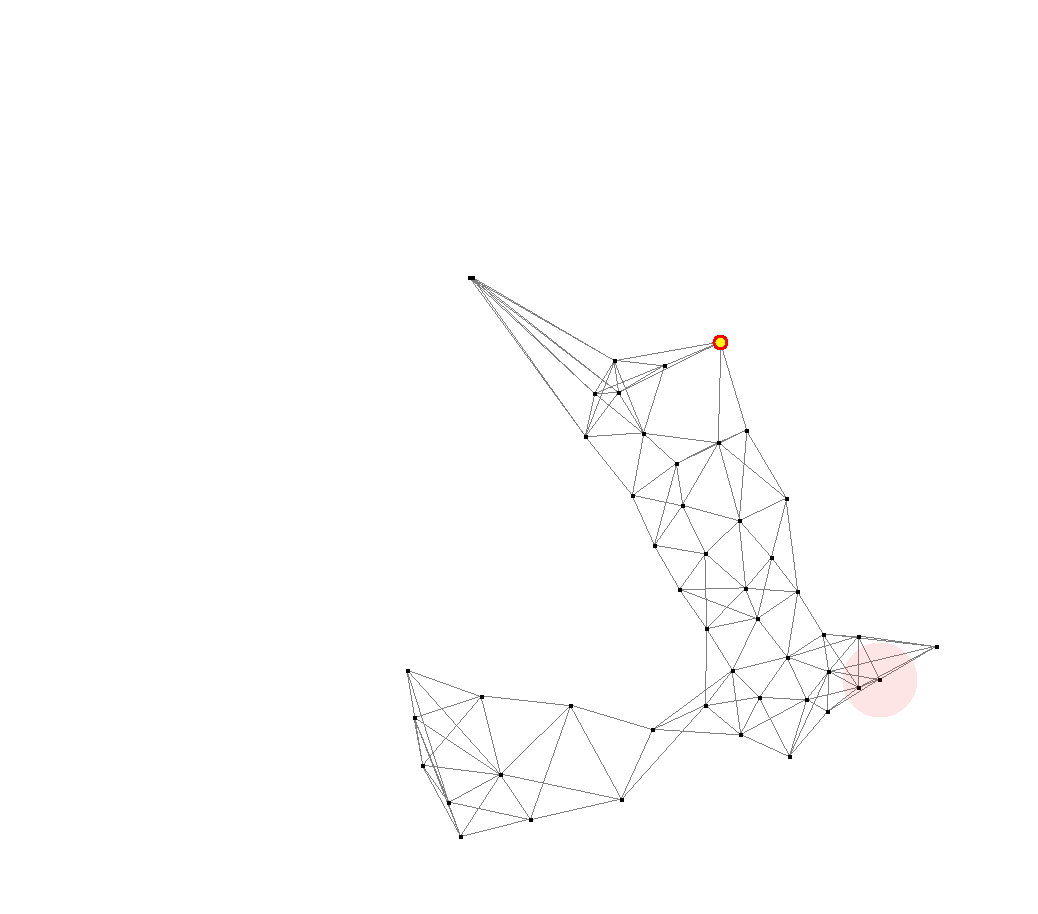
\includegraphics[width=0.3\textwidth]{img/moment-b.png}
	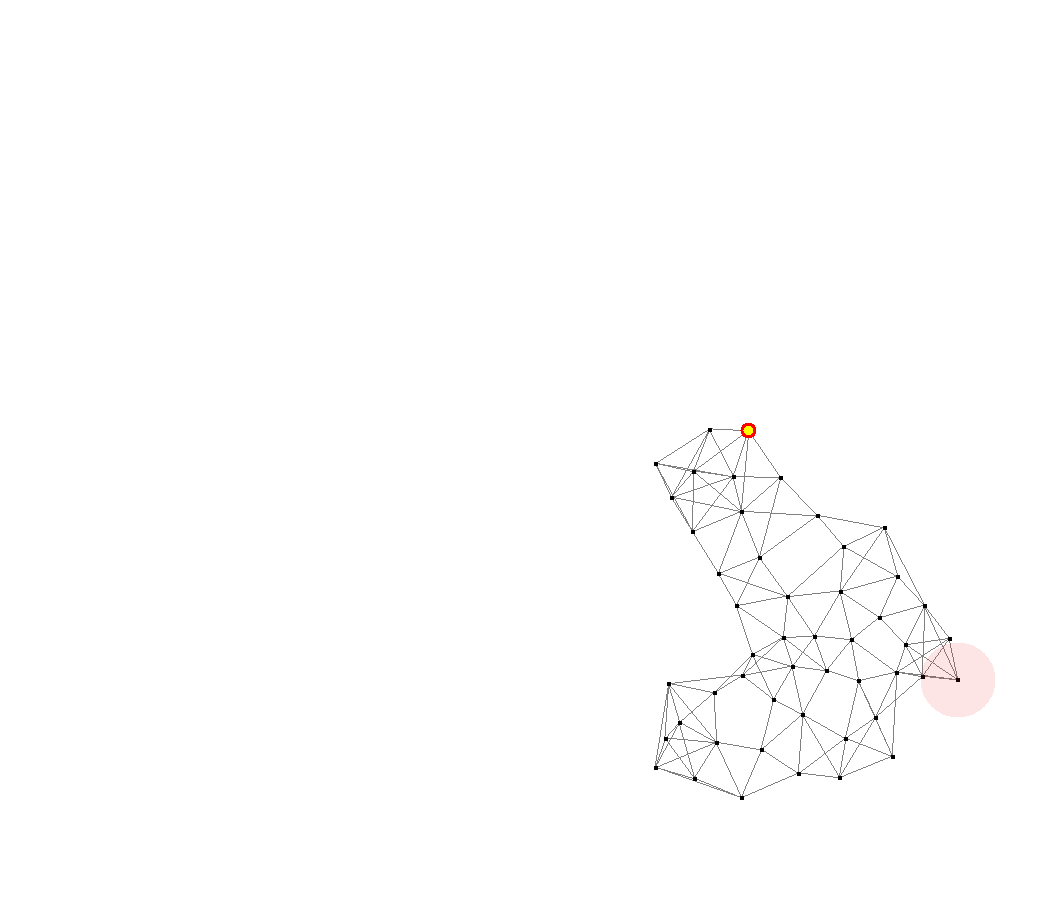
\includegraphics[width=0.3\textwidth]{img/moment-c.png}
}
\end{frame}
\begin{frame}{Open Challenges}
	\begin{itemize}
		\item \textbf{Curse of dimensionality}
		\begin{itemize}
			\item Exponential growth in computational complexity from an increase in state and action
			dimensions. Also a challenge for single-agent problems. 
			\begin{itemize}
				\item Partially handled by homogeneous policies 
			\end{itemize}
		\end{itemize}
		\item \textbf{Specifying a good (learning) objective}
		\begin{itemize}
			\item Agent returns are correlated and cannot be maximized independently.
			\begin{itemize}
				\item Multi-agent credit assignment problem (how can I know if my action was good?)
			\end{itemize}
		\end{itemize}
		\item \textbf{Need for coordination}
		\begin{itemize}
			\item Agent actions affect other agents and could confuse other agents (or herself) if not
			careful. Also called destabilizing training
		\end{itemize}
		\item \textbf{No formal guarantees}
		\begin{itemize}
			\item No formal guarantees on convergence, stability, or optimality
		\end{itemize}

	\end{itemize}
\end{frame}
\begin{frame}{Conclusion}
	\begin{itemize}
		\item Multi-Agent Reinforcement Learning is a very active research field
		\item From Single to Multi-Agent RL, different axes to consider:
		\begin{itemize}
			\item Training strategy: centralised or decentralised
			\item Policy constraints: homogeneous or heterogeneous
			\item Agent population: few or many
			\item \dots
		\end{itemize}
		\item Several techniques have been proposed to handle the complexity of the problem
		\begin{itemize}
			\item MAPPO, Mean-Field RL, COMA, \dots
		\end{itemize}
		\item No one size fits all solution 
		\begin{itemize}
			\item Some handle only cooperative problems
			\item Other works only with a few agents
			\item \dots
		\end{itemize}
		\item My hope: a general framework for MARL (like the one for RL)
	\end{itemize}
\end{frame}
%===============================================================================
\section*{}
%===============================================================================

%/////////
\frame{\titlepage}
%/////////

%===============================================================================
\section*{\refname}
%===============================================================================

%%%%%%%%%%%%%%%%%%%%%%%%%%%%%%%%%%%%%%%%%%%%%%%%%%%%%%%%%%%%%%%%%%%%%%%%%%%%%%%%
\end{document}
%%%%%%%%%%%%%%%%%%%%%%%%%%%%%%%%%%%%%%%%%%%%%%%%%%%%%%%%%%%%%%%%%%%%%%%%%%%%%%%%
